\documentclass[11pt,a4paper]{article} % Type de documents

% Importation des paquets nécessaire à la compilation du projet
\usepackage{graphicx}
\usepackage{xcolor}

\usepackage{csquotes}
\usepackage [english]{babel}
\usepackage{fancyhdr}

\usepackage{algpseudocode}
\usepackage{algorithm}
\usepackage{amsmath}
\usepackage{float}

\usepackage{siunitx}
\usepackage[
backend=biber,
style=alphabetic,
sorting=ynt
]{biblatex}

\usepackage{xcolor} % Required for custom colors
\usepackage{hyperref} % Required for hyperlinks

\usepackage{geometry}

% Spécifiez les marges ici
\geometry{left=2cm, right=2cm, top=2cm, bottom=2cm}

% Define custom colors
\definecolor{linkcolor}{HTML}{0000FF} % Blue color for links
\hypersetup{
    colorlinks=true,
    linkcolor=linkcolor, % Set the color of internal links
    urlcolor=linkcolor   % Set the color of URLs
}



\addbibresource{references.bib}
\nocite{*}

\begin{document}

\begin{titlepage}

\raggedleft

\includegraphics[scale=0.2]{images/logo.jpg}\\

% Input text above title if you wish 
\vspace{3cm}
\begin{center}
\newcommand{\HRule}{\rule{\linewidth}{0.5mm}}
\textsc{\Large S4.A.01 2023-24}\\[2.0mm]
\textsc{\Large Computer Science Bachelor, A}\\[2.0mm]
\vspace{0.8cm}
    \HRule\\[0.4cm]
    {\huge\bfseries Information theory}\\[0.4cm] 
    \HRule\\[1.5cm]
    
    \begin{minipage}{0.4\textwidth}
        \begin{flushleft}
            \large
            \textit{Authors:}\\
            \text{}\\
            \text{GODINAT Caetano, PICAURON Adam, DAUGE Alexis}\\
            \text{(Group 21)}\\
        \end{flushleft}
    \end{minipage}
        ~
    \begin{minipage}{0.4\textwidth}
        \begin{flushright}
            \large
            \text{ } \\
        \end{flushright}
    \end{minipage}
\mbox{}
\vfill

\date{March 2024}

\end{center}
\end{titlepage}

\newpage
\thispagestyle{empty}

\setcounter{tocdepth}{3}

% Table des matières mise à jour automatiquement
\renewcommand{\contentsname}{Table of Contents}
\tableofcontents
\newpage

\setcounter{page}{1}
\parskip = \baselineskip
\newpage

% Les sections (et leur sous sections) correspondantes au plan mis en place dans la table des matières
\section{Introduction}

In today's interconnected world, the abundance of information presents a significant challenge in measuring its transmission capacity. Enter Claude Elwood Shannon, a mathematician whose groundbreaking article revolutionized the field of communication and information. Shannon's Mathematical Theory of Communication introduced a systematic framework for quantifying the flow of information through a given system. In this article, we try to apply Shannon's theory to two different fields information compression and cryptography to see whether the outcomes align with our expectations.

\begin{figure}[!h]
\centering
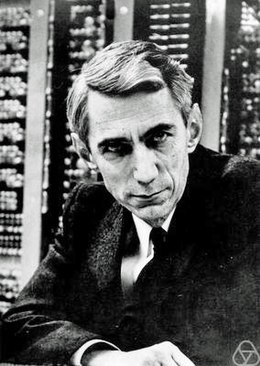
\includegraphics[scale=0.7]{images/shanon.jpg}
\caption{Claude Shannon around 1963 \cite{wiki_sha}}
\label{shannon}
\end{figure}

\newpage

\section{Applications}

\subsection{Data compression}

A "lossless" compression algorithm is defined as any coding procedure whose objective is to represent a certain quantity of information using or occupying a smaller space allowing the exact reconstruction of the original data.

\subsubsection{Introduction to Huffman's compression}

Invented by David Albert Huffman and published in 1952, Huffman coding is a lossless data compression algorithm. It uses a variable-length code to represent a symbol in the source message. The compressed binary code is determined by estimating the probability of occurrence of the symbols linked to the branches of a binary tree.

There are several implementations of this binary tree: \cite{wiki_huffman}

\begin{itemize}
 \item Static : Each byte has a predefined code, the tree does not need to be transmitted ;
 \item Semi-Adaptive : Calculates the occurrence of each byte, the tree needs to be transmitted ;
 \item Adaptive : Uses a known tree modified dynamically as the stream is compressed according to the symbols previously encountered ;
\end{itemize}

For the purposes of this report, we will be implementing the semi-adaptive

\subsubsection{Principles}age

The string we are going to compress is \textbf{"Information theory"}, and its binary code is as follows: \textbf{01001001 01101110 01100110 01101111 01110010 01101101 01100001 01110100 01101001 01101111 01101110 00100000 01110100 01101000 01100101 01101111 01110010 01111001}

Needless to say, it's a lot and that's why we're trying to compress it using our algorithm.
The principle is as follows: we calculate the occurrence of each letter in the source (the character string), then we sort this list in ascending order of occurrence. This list can be used to build a binary tree in the following "Bottom-Up" way:
\begin{figure}[H]
    \centering
    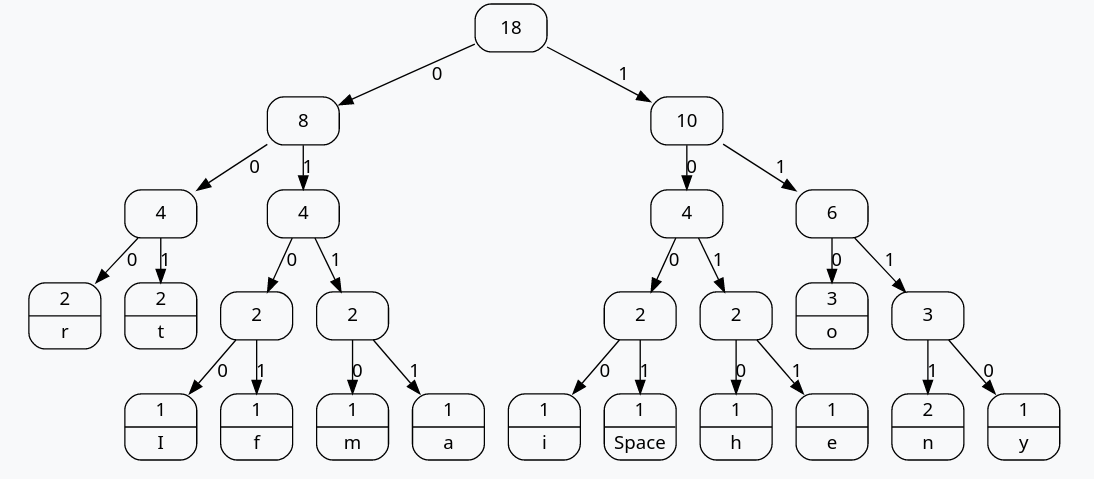
\includegraphics[width=0.5\linewidth]{images/HuffmanBT.png}
    \caption{Enter Caption}
    \label{fig:huffman-bt}
\end{figure}

By traversing this tree from node to node to reach the nodes corresponding to the letters we are looking for, we can find the compressed binary code assigned to them. The nodes on the left have a metric of 0 on their branch and a metric of 1 for the branches on the right (refer to the diagram of the previous tree). This gives the following binary code for the chosen source: \textbf{1101100100101110111101100100111011000011000000010111100} ... Much better, isn't it?

In order to decompress our compressed source and retrieve the exact starting data, we need to transmit the tree when communicating the source. (In Python we pass the object created for the tree).

As each node corresponds to a letter and has a weight on the branch linking it to other nodes, we can recover the exact source by simply traversing the tree and obtaining the \textbf{"Information theory"} string again.

\subsubsection{Limits and Performances}

For any source \textbf{X} with a Shannon entropy noted \textbf{H(X)} has an average length \textbf{L} of a codeword obtained by Huffman coding verified the following property: 

$H(X) <= L < H(X) + 1$.

The previous relationship shows that Huffman's algorithm approximates the entropy of our source and this may not be very interesting in the case of high entropy, where an overhead of 1 bit becomes significant. 

One solution to this problem is to work on blocks of \textbf{n} symbols. We then show that we can get closer to the entropy: 

$ H(X)\leq L<H(X)+{\frac {1}{n}} $

but the process of estimating probabilities becomes more complex and costly.
\subsection{Forward error correcting}

In telecommunications and computing, forward error correction (FEC) is a digital signal processing technique used to control errors in data transmission over unreliable or noisy communication channels, as well as to independently increase data reliability at the receiver to ensure high quality.

FEC improves bit error rate efficiency in communication systems, but involves additional digital processing, making it more expensive in terms of cost and spectral efficiency. The balance between these two elements needs to be taken into account in systems.

This is achieved by introducing redundant data using error-correcting codes (ECC) before the message is transmitted.  Without redundancy, every piece of data in the message is essential to its understanding. Any error in the message can therefore change its meaning.  The aim is to ensure that errors do not compromise the overall understanding of the message, and do not trigger a request for a re-transmission of the message by the receiver, thereby reducing channel traffic by more than a factor of two.

\subsubsection{Introduction to error correction code}

The problems encountered by modern industry are very diverse, all offering multiple techniques used for error-correcting codes. In some cases, such as data transmission over the Internet, the ECC's role is limited to error detection. In other cases, such as the TCP protocol on the transport layer of the OSI model, when an error is detected during message transmission, it is corrected by retransmitting the message. The techniques listed here are just a few of a sea of others, and today we're going to take a look at a very special technique known for its effectiveness : \textbf{Convolutional correctors}

The special feature of a convolutional ECC is that its output depends on the current symbol to be coded, as well as the previous symbol and the result of coding the previous symbol, unlike block codes, which process each block of information independently of the others.

For the purposes of this report, we will confine ourselves to the case of discrete communication channels, which are nothing other than binary channels transmitting only 0 or 1, i.e. bits of information.

\subsubsection{Convolutional encoding}

\begin{figure}[H]
    \centering
    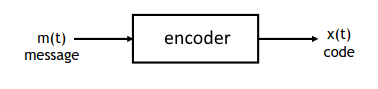
\includegraphics[width=0.5\linewidth]{images/encodeur_schem.png}
    \caption{Communication encoder diagram}
    \label{fig:encoder-diagram}
\end{figure}

A convolutional encoder is a finite state machine, and its state diagram can be represented as a lattice (the temporal equivalent of a state diagram). All states are arranged in columns to represent a state at time \textbf{t}, where \textbf{m(t)} and \textbf{x(t)} are discrete signals whose samples are binary. These states are linked to the same sets of states representing time t+1, in accordance with the transition table.

\begin{figure}[H]
    \centering
    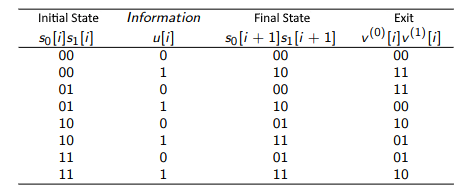
\includegraphics[width=0.5\linewidth]{images/transitionTable.png}
    \caption{Transition table with i for the clock time}
    \label{fig:transition-table}
\end{figure}

If the encoder is a linear system, \textbf{x(t)} can be generated by a convolution product:
\[ x_{j} = \sum_{i=0}^M g_{i}m_{j-i} \]

In order to carry out a binary convolution coding we will set some parameters:
\begin{itemize}
     \item $g_{i} = 0 \rightarrow$ connection absent
     \item $g_{i} = 1 \rightarrow$ connection present
     \item $K \rightarrow$ Constraint length (number of sampling instants during which a message bit participates in the elaboration of the output)
\end{itemize}

This is a so-called sliding window coding where there are two integers \textit{m} (for memory) and \textit{a} (for anticipation) such that the index symbol n of the coded sequence depends only on the finite source block between the indices $n - m$ and $n + a$.
\begin{figure}[H]
    \centering
    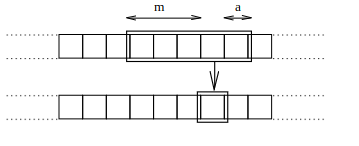
\includegraphics[width=0.5\linewidth]{images/register.png}
    \caption{Shift register}
    \label{fig:shift-register}
\end{figure}

For 1/2-rate 2-memory convolutional encoder we take M = 2, then we have K = M + 1 = 3 with an output interleaving n = 2, so using the above formula we obtain the following generator polynomials: $g_{1} = [1, 1, 1]$ and $g_{2} = [1, 0, 1]$.

All these parameters allow us to obtain the following logic diagram, enabling convolutional coding of our ECC: 
\begin{figure}[H]
     \centering
     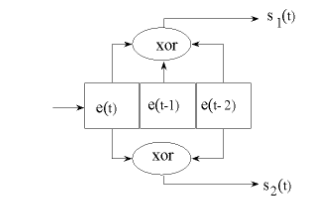
\includegraphics[width=0.5\linewidth]{images/logical_circuit.png}
     \caption{Data transmission in a convolutional encoder with a shift register and exclusive ORs}
     \label{fig:logical-circuit}
\end{figure}

Using this schema and XORing according to the connections said to be absent or present on the register undergoing a shift along the chain to be encoded we obtain:
\begin{itemize}
 \item Initial string : \textbf{1010}
 \item Encoded string: \textbf{11100010}
\end{itemize}

We therefore observe the presence of redundancy, as explained in the introduction, with a redundancy bit for each bit of the initial character string, which we'll use for decoding.

Before we start decoding, as we are working on noisy discrete channels, we will apply noise to the character string to check that our appended code is working correctly. Our message therefore becomes $\rightarrow$ \textbf{11100011}


\subsubsection{Decoding with Viterbi algorithm}

The Viterbi algorithm is based on the dynamic programming paradigm. We start from a starting state (default 00) and seek to find the path from the starting state whose output has the same length and is as close as possible to the message to be decoded. To apply this notion of proximity, we use the Hamming distance, which counts the number of different bits between two messages of the same finite or infinite length. 

This Hamming distance can be translated into the following pseudo-code:

\begin{algorithm}[H]
\begin{algorithmic}
\Function{Hamming distance}{$\text{s1}, \text{s2}$}
    \If{$\text{len}(\text{s1}) \neq \text{len}(\text{s2})$}
        \State \Return "Strings must be of equal length"
    \EndIf
    \State $\text{dist} \gets 0$
    \For{$i \gets 0$ \textbf{to} $\text{len}(\text{s1}) - 1$}
        \If{$\text{s1}[i] \neq \text{s2}[i]$}
            \State $\text{dist} \gets \text{dist} + 1$
        \EndIf
    \EndFor
    \State \Return $\text{dist}$
\EndFunction
\end{algorithmic}
\end{algorithm}

In response to the dynamic programming paradigm, the Viterbi algorithm can be represented in ways other than as a lattice. For the sake of simplicity, it will be presented in the form of a binary tree, so that we can create a history of all possible paths and perform a recursion to calculate the metric of each path from that of each branch, and reconstruct the message to be decoded.

\begin{figure}[H]
     \centering
     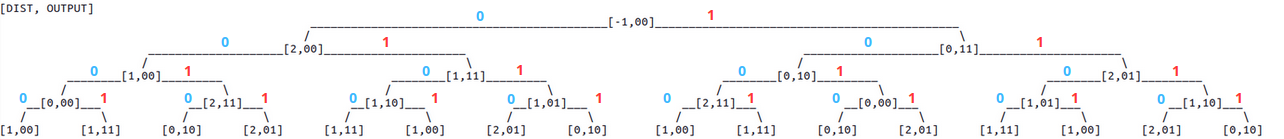
\includegraphics[width=1\linewidth]{images/BT_ECC_CV.png}
     \caption{Representation of the binary tree of the Viterbi lattice}
     \label{fig:bt-ecc-cv}
\end{figure}

Using the transition table in figure n°\ref{fig:transition-table}, we can move from one state to another and retrieve the new state, as well as the output bits, all thanks to the input bits which are 0 for the nodes on the left and 1 for the nodes on the right. A state is in fact a pair of bits resulting from the concatenation of the initial bit and the redundancy bit. If we go back up our tree, all we have to do is concatenate the input bits to reconstitute the message, even if it has been noisy. We know which is the safest path to take thanks to the distances noted above.

\begin{figure}[H]
     \centering
     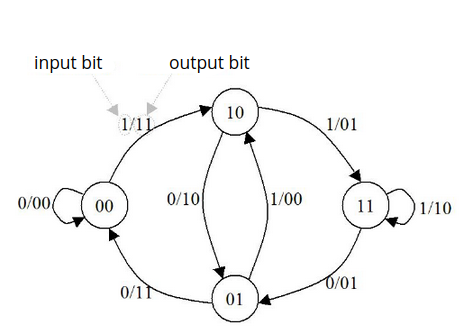
\includegraphics[width=0.5\linewidth]{images/logical_circuit_v2.png}
     \caption{State diagram of a convolutional encoder with 2 memories and 1/2 rate}
     \label{fig:logical_circuit_v2}
\end{figure}

Now, we can retrieve the correct message that is \textbf{1010}.

\newpage
\subsection{Cryptography}
\subsubsection{Introduction}
In a traditional definition of security of a cryptography scheme, one usually defines a game that characterizes the capabilities of a (hypothetical) adversary. A cryptography scheme is defined to be secure if no computationally feasible strategy allows the adversary to win the game with non-negligible probability (or advantage), for reasonable notions of feasible and negligible.
\cite{maurer2011constructive}

\paragraph{Important Elements of Cryptography}
\paragraph{Plain-text}
Original text that is immediately intelligible and can therefore be directly, without the need for deciphering.
\cite{ramet_r3.09}

\paragraph{Encrypting}
An operation that substitutes a plain text with an unintelligible text that cannot be understood by anyone who does not possess the key. Inoperable by anyone who doesn't have the key.

\paragraph{Ciphertext}
Message made unintelligible through encryption, which can only be and used only by those in possession of the encryption key.

\paragraph{Decryption}
Reverse operation of a reversible encryption, allowing an authorized in possession of the key, to restore a ciphertext in clear text.

\paragraph{Types of Cryptography}
There are two types of Cryptography: symmetric key Cryptography and asymmetric key Cryptography, both still in use today, but they have different applications due to their different qualities.

\paragraph{Symmetric Cryptography}
Symmetric Cryptography is the first one to appear, as it is a basic concept, it is as if we had a key to open a chest. In Cesar cipher is the number of shifts we will do on the alphabet to write and read the plain-text and the ciphertext respectively. The key being the most essential element in computational Cryptography, it can be almost anything that is information, a string of text, numbers, an image, etc… That information being processed by a Cryptography algorithm it can then encode or decode Cryptographic data. Today symmetric Cryptography is used in cases where we need fast service using not much resources and not needing to share the secret key often. Such qualities interest banks for example. There are multiple symmetric cryptography algorithms such as AES, DES, 3DES, and Blowfish. All of them are based on the Feistel Network except for AES which uses a Substitution and Permutation Network.

\paragraph{Asymmetric Cryptography}
ECC (Elliptic-curve-Cryptography) Elliptic Curve Cryptography Overview Elliptic Curve Diffie Hellman A 384 bits ECC key has the same level of security as a 7680 bit RSA key, it is considered to be a Top Secret level of security by many governments such as the USA Government Shannon Information Theory and Cryptography.

\subsubsection{Advanced Encryption Standard (AES)}
AES was invented by two Belgians, Joan Daemen and Vincent Rijmen in 1998 and submitted to the National Institute of Standards and Technology (NIST) in 2001 in order to replace the DES (Data Encryption Standard) which was starting to get outdated. It uses a key of 3 different lengths 128, 192, and 256 bits.
\cite{wiki_aes}


\paragraph{Variables}\cite{nist_aes}
\begin{itemize}
    \item [$-$] \textbf{state} Intermediate result of the AES block cipher that is represented as a two-dimensional array of bytes with four rows and Nb columns.
    \item [$-$] \textbf{keys} the key schedule generated by the key expansion algorithm
\end{itemize}
\paragraph{Constants}\cite{nist_aes}
\begin{itemize}
    \item [$-$] \textbf{s\_box} A non-linear substitution table used in SUBBYTES and KEYEXPANSION to perform a one-to-one substitution of a byte value.
    \item [$-$] \textbf{inv\_s\_box} A non-linear substitution table with the inverse values of the S-box used for the decryption.
    \item [$-$] \textbf{mix\_columns} A fixed matrix used on the MIXCOLUMNS
    \item [$-$] \textbf{inv\_mix\_columns} The matrix with the hexadecimal values of mix\_columns used in INVMIXCOLUMNS
    \item [$-$] \textbf{rcon} Is the key expansion round constants used on the KEYEXPANSION
\end{itemize}
\paragraph{Functions}\cite{nist_aes}
\begin{itemize}
    \item [$-$] \textbf{SUBBYTES} Takes the state as the parameter and applies the s\_box to each byte independently.
    \item [$-$] \textbf{SHIFTROWS} Takes the state as the parameter and transforms the state shifting the last three rows with different offsets (2nd row has 1 offset, 3rd row has 2 offsets, and 4th row has 3 offsets)
    \item [$-$] \textbf{MIXCOLUMNS} Takes the state as the parameter and each column is multiplied by the Mix Columns matrix. But the multiplication is done in the Galois Field. Which means that the sum is done with the XOR operation and the multiplication is done with the AND operation.
    \item [$-$] \textbf{KEYEXPANSION} Takes the key as the parameter, the routine that generates the round keys from the key.
    \item [$-$] \textbf{ADDROUNDKEY} Takes the state and round key as the parameters and transforms the state by performing an XOR operation on the state with the round key.
    \item [$-$] \textbf{CIPHER} Takes the plain text and the key as arguments and perform the AES algorithm using the functions SUBBYTES, SHIFTROWS, MIXCOLUMNS, KEYEXPANSION and ADDROUNDKEY.
    \item [$-$] \textbf{INVCIPHER} Takes the cipher text and makes the reverse operation as CIPHER.
\end{itemize}

\paragraph{AES Algorithm}\cite{nist_aes}
\begin{algorithm}[H]
\caption{CIPHER Algorithm}
\begin{algorithmic}[1]
\Procedure{CIPHER}{$plain\_text: list[int], key: list[int]$}
    \State $state \gets 4 \times 4$ matrix of zeros
    \For{$i \in [0, 4)$}
        \For{$j \in [0, 4)$}
            \If{$i*4+j < \text{len}(plain\_text)$}
                \State $state[j][i] \gets plain\_text[i*4+j]$
            \EndIf
        \EndFor
    \EndFor
    \State $keys \gets \text{KEYEXPANSION}(key)$
    \State $state \gets \text{ADDROUNDKEY}(state, keys[0])$
    \For{$i \in [1, 10)$}
        \State $state \gets \text{SUBBYTES}(state)$
        \State $state \gets \text{SHIFTROWS}(state)$
        \State $state \gets \text{MIXCOLUMNS}(state)$
        \State $state \gets \text{ADDROUNDKEY}(state, keys[i])$
    \EndFor
    \State $state \gets \text{SUBBYTES}(state)$
    \State $state \gets \text{SHIFTROWS}(state)$
    \State $state \gets \text{ADDROUNDKEY}(state, keys[10])$
    \State \Return $[state[i][j] \text{ for } i \in [0, 4) \text{ for } j \in [0, 4)]$
\EndProcedure
\end{algorithmic}
\end{algorithm}

\paragraph{Why is AES so hard to break}
For symmetric Cryptography we have three properties that measures if a cryptography system is secure or not.
\paragraph{Confusion and Diffusion}\cite{ramet_r3.09}
Confusion is when there is no statistical property that can be deduced from the ciphertext and Diffusion is when a change on the plain text changes the majority of the ciphertext.

\paragraph*{Example of Diffusion and Confusion in AES}

\textbf{Plain-text 1:} Hello World!

\textbf{Ciphertext 1:} \\
{\small\texttt{0101111111001111111111000010100001101100110001011011001010001000\\1110101000000011000011101000100010011000110110001100011001000010}}

\textbf{Plain-text 2:} Hallo World!

\textbf{Ciphertext 2:} \\
{\small\texttt{0100011001111001011111000100101000100100010011110101001100010100\\1011001010110010110110001010010101111111101101011110011110100111}}

\paragraph*{Analysis}

As observed, changing one letter in the plain-text resulted in a completely different ciphertext. This demonstrates the \textbf{Diffusion} property of AES. Moreover, due to the significant changes in the ciphertext, it becomes challenging to deduce statistical properties from these two messages, showcasing the \textbf{Confusion} property.

\paragraph{Key robustness} 
When is hard to find or enumerate all possibilities of key.

If the algorithm has the Diffusion and the Confusion properties, the only way to find the key would be by trying every combination of key. Which means that to find the key it would be needed to try 2 to the power 128 possibilities.

\paragraph{Why is AES better than DES}
\begin{itemize}
    \item AES provides stronger security compared to DES.
    \item AES is faster and more efficient in terms of computation compared to DES.
    \item AES has been subjected to more scrutiny and analysis than DES, making it more reliable.
\end{itemize}

\subsubsection{Elliptic-curve Cryptography (ECC)}
ECC (Elliptic-curve Cryptography) is a public-key cryptography algorithm based on the algebraic structure of elliptic curves over finite fields. It offers a high level of security with relatively short key sizes compared to other public-key cryptography algorithms like RSA. Elliptic Curve Diffie-Hellman (ECDH) is a key exchange protocol based on ECC, and it provides a secure way for two parties to establish a shared secret over an insecure channel. Although ECC is more secure than RSA, a 384 bit ECC key is equivalent to a 7680 RSA key for example.

\paragraph{How does Elliptic-curve Cryptography works}\cite{pierce_ecdh}
\paragraph{Curve}
An Elliptic-curve is defined by 
\begin{equation*}
y^2 = x^3 + ax + b
\end{equation*}
where $a$ and $b$ are constants. And the curve looks like this.

\begin{figure}[H]
\begin{minipage}{0.5\textwidth}
  \centering
  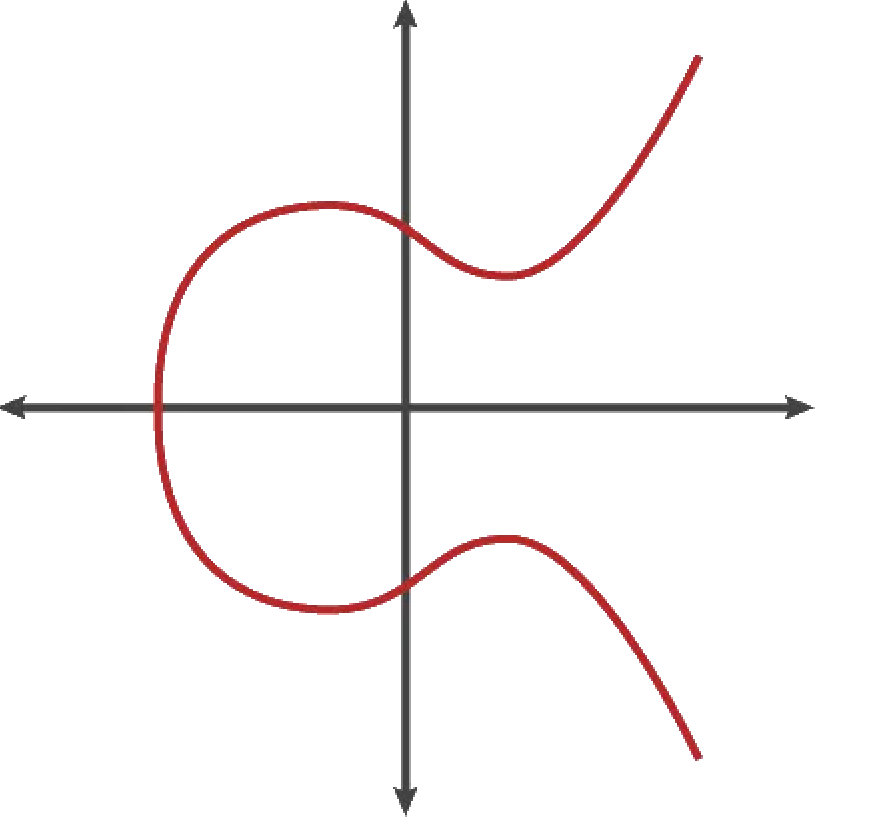
\includegraphics[width=\linewidth]{images/curve.png}
  \caption{Elliptic-curve.}
  \label{fig:Elliptic curve}
\end{minipage}%
\begin{minipage}{0.5\textwidth}
An Elliptic-curve is defined by $y^2 = x^3 + ax + b$ where $a$ and $b$ are constants. This figure illustrates the general shape of an elliptic curve.
\end{minipage}
\end{figure}

\paragraph{Addition}
The addition operation consists of finding a 3rd point on the curve. In the example we see the following operation:
\begin{equation}
P + Q = R
\end{equation}
When we draw a line that passes through $P$ and $Q$ we get $-R$ and through the property of symmetry of elliptic curves, we can find $R$.

\begin{figure}[H]
\begin{minipage}{0.5\textwidth}
  \centering
  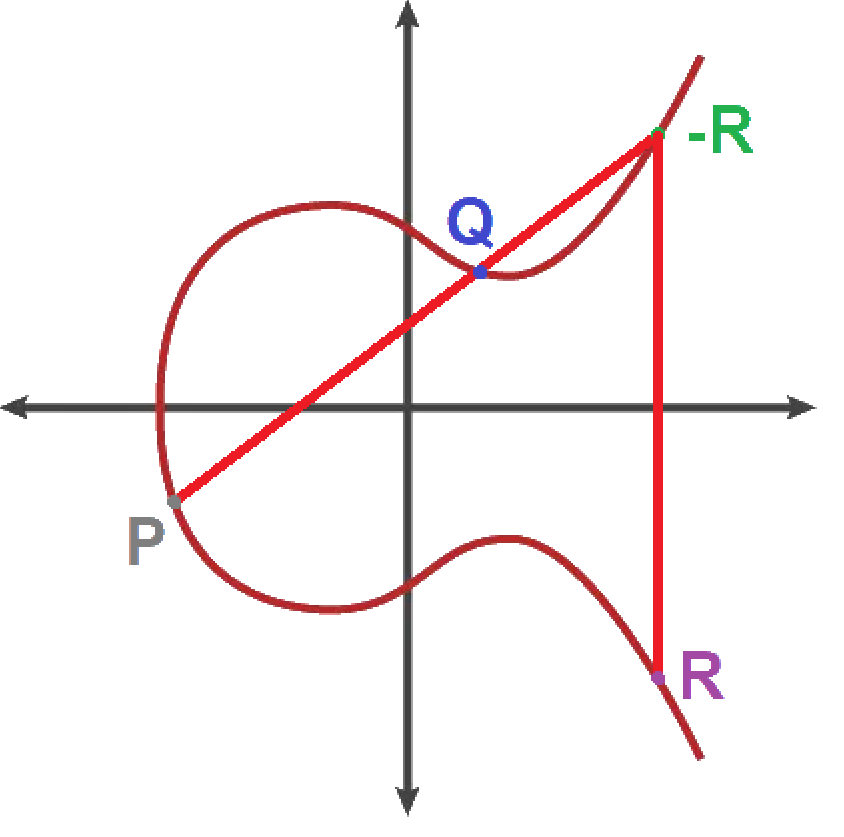
\includegraphics[width=\linewidth]{images/point_addition.png}
  \caption{Point addition in ECC.}
  \label{fig:point addition in ECC}
\end{minipage}%
\begin{minipage}{0.5\textwidth}
The addition operation consists of finding a third point on the curve. This figure illustrates the geometric interpretation of point addition in ECC.
\end{minipage}
\end{figure}

\paragraph{Multiplication}
The multiplication operation consists of adding a point $k$ times.
\begin{equation}
kP = P + P + \ldots + P 
\end{equation}
When adding a point to itself on a curve, the line drawn is the tangent to the curve at that point, $P$.

\begin{figure}[H]
\begin{minipage}{0.5\textwidth}
  \centering
  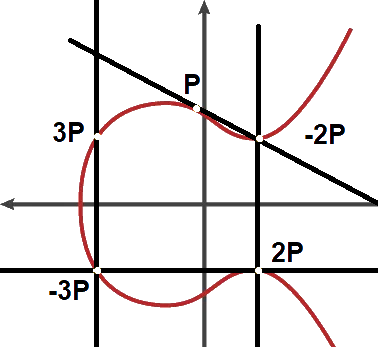
\includegraphics[width=\linewidth]{images/mult.png}
  \caption{Scalar Multiplication.}
  \label{fig:Scalar Multiplication}
\end{minipage}%
\begin{minipage}{0.5\textwidth}
The multiplication operation consists of adding a point $k$ times. This figure illustrates the concept of scalar multiplication in ECC.
\end{minipage}
\end{figure}

\paragraph{Implementation}
We will need to Implement two functions, add (make the addition of points), multiply(multiply a point).

The multiplication function will be a simple function of repeating an addition n times.
For the addition it wont be as simple.
So the algorithm will implement this logic.
\begin{enumerate}
    \item If one of the points is the point at infinity (represented as (0, 0)), then adding it to another point returns the other point.
    \item If the points are additive inverses (negatives) of each other, their sum is the point at infinity.
    \item If the points are distinct, calculate the slope of the line passing through them.
    \begin{equation}
    s = \frac{{Y_P - Y_Q}}{{X_P - X_Q}}
    \end{equation}
    \begin{equation}
    X_R = s^2 - (X_P - X_Q)
    \end{equation}
    \begin{equation}
    Y_R = s(X_P - X_R) - Y_P
    \end{equation}
    \item If the points are the same, calculate the slope of the tangent line to the curve at that point.
    \begin{equation}
    s = \frac{{3X_{P}^{2} + a}}{{2Y_{P}}}
    \end{equation}
    \begin{equation}
    X_R = s^2 - 2X_P
    \end{equation}
    \begin{equation}
    Y_R = s(X_P - X_R) - Y_P
    \end{equation}
\end{enumerate}

\begin{algorithm}[H]
\caption{Add two points on the curve}
\begin{algorithmic}[1]
\Procedure{Add}{$p, q$}
    \If{$p = (0, 0)$}
        \State \textbf{return} $q$
    \EndIf
    \If{$q = (0, 0)$}
        \State \textbf{return} $p$
    \EndIf
    \If{$p[0] = q[0]$ \textbf{and} $p[1] = -q[1]$}
        \State \textbf{return} $(0, 0)$
    \EndIf
    \If{$p \neq q$}
        \State $l \gets (q[1] - p[1]) \cdot (q[0] - p[0])^{-1} \mod p \, \% \, p$
    \Else
        \State $l \gets (3 \cdot p[0]^2 + a) \cdot (2 \cdot p[1])^{-1} \mod p \, \% \, p$
    \EndIf
    \State $x \gets (l^2 - p[0] - q[0]) \mod p \, \% \, p$
    \State $y \gets (l \cdot (p[0] - x) - p[1]) \mod p \, \% \, p$
    \State \textbf{return} $(x, y)$
\EndProcedure
\end{algorithmic}
\end{algorithm}

\paragraph{What makes ECC secure}

For a asymmetric Cryptography system the most important thing is to create a common key between two parts while not revealing their own private key, so it must be easy to calculate a public key from the private key but hard to make the reverse operation from the public key, that is called a trapdoor function.

To show how ECC works let's try a practical example:
\begin{figure}[H]
  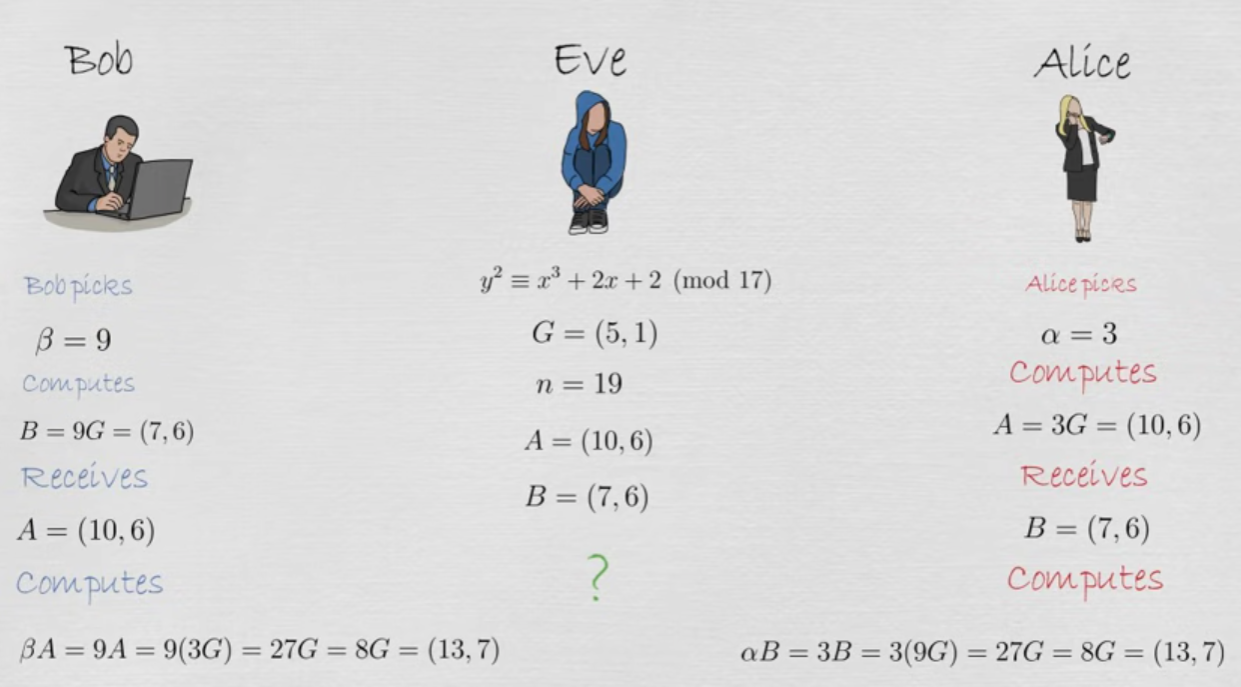
\includegraphics[width=\linewidth]{images/expl.png}
  \caption{Practical example of ECC.}\cite{pierce_ecdh}
  \label{fig:Practical example of ECC}
\end{figure}
In this scenario, Eve, acting as the intermediary, managed to obtain some information, albeit incomplete. However, she lacks the critical data necessary to compute the private keys. The inherent complexity of elliptic curves ensures that deriving either the private key $\beta$ (Bob's private key) or the private key $\alpha$ (Alice's private key) in ECC solely from a point on the curve is highly challenging.
This is a simple example, as there are standard parameters for the curb such as sect571k1. \cite{secg2010}


\subsubsection{Cryptography and Shannon Information Theory} \cite{shannon1948mathematical}

In The Theory of Communication the encoding and decoding are operations made by the transmitter and the receiver both will be called transducers.

And according to the Theorem 9 it is not possible for the channel to transmit at an average rate greater than: $\frac{C}{H}-\epsilon$

For the AES cryptography system the limit is calculated like this:

First let's calculate the capacity C of the system.
As in ASCII we have a set of characters of length 128, let's name it A* and every character (or symbol) is coded in 7 bits they have the same time of encoding or decoding.
Let's define \textbf{z} which is theoretical time that a transducer takes to encode or decode a character
\begin{enumerate}
    \item Build the system for the calculations
        \begin{figure}[H]
          \centering
          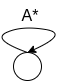
\includegraphics[width=0.15\linewidth]{images/system.png}
          \caption{cryptosystem schema.}
          \label{fig:cryptosystem}
        \end{figure}
        The matrix defining the system above will look like:
        $\left|({128*W^{z}})-1\right| = 0$
    \item Find the determinant of the equation, in this case as the matrix is a singleton matrix, the determinant of the matrix is itself.
    \item Solve ${128*W^{z}}-1 = 0$ to find $W$
    \item Calculate the capacity $C = logW$
\end{enumerate}

Secondly, H is defined as the bits per symbol as said before:
$H = 7$

Finally calculate the maximum average rate of the channel $\frac{C}{H}$
\begin{equation}
    \frac{logW}{7}
\end{equation}
\newpage
\section{Applications}

\subsection{Data compression}

A "lossless" compression algorithm is defined as any coding procedure whose objective is to represent a certain quantity of information using or occupying a smaller space allowing the exact reconstruction of the original data.

\subsubsection{Introduction to Huffman's compression}

Invented by David Albert Huffman and published in 1952, Huffman coding is a lossless data compression algorithm. It uses a variable-length code to represent a symbol in the source message. The compressed binary code is determined by estimating the probability of occurrence of the symbols linked to the branches of a binary tree.

There are several implementations of this binary tree: \cite{wiki_huffman}

\begin{itemize}
 \item Static : Each byte has a predefined code, the tree does not need to be transmitted ;
 \item Semi-Adaptive : Calculates the occurrence of each byte, the tree needs to be transmitted ;
 \item Adaptive : Uses a known tree modified dynamically as the stream is compressed according to the symbols previously encountered ;
\end{itemize}

For the purposes of this report, we will be implementing the semi-adaptive

\subsubsection{Principles}age

The string we are going to compress is \textbf{"Information theory"}, and its binary code is as follows: \textbf{01001001 01101110 01100110 01101111 01110010 01101101 01100001 01110100 01101001 01101111 01101110 00100000 01110100 01101000 01100101 01101111 01110010 01111001}

Needless to say, it's a lot and that's why we're trying to compress it using our algorithm.
The principle is as follows: we calculate the occurrence of each letter in the source (the character string), then we sort this list in ascending order of occurrence. This list can be used to build a binary tree in the following "Bottom-Up" way:
\begin{figure}[H]
    \centering
    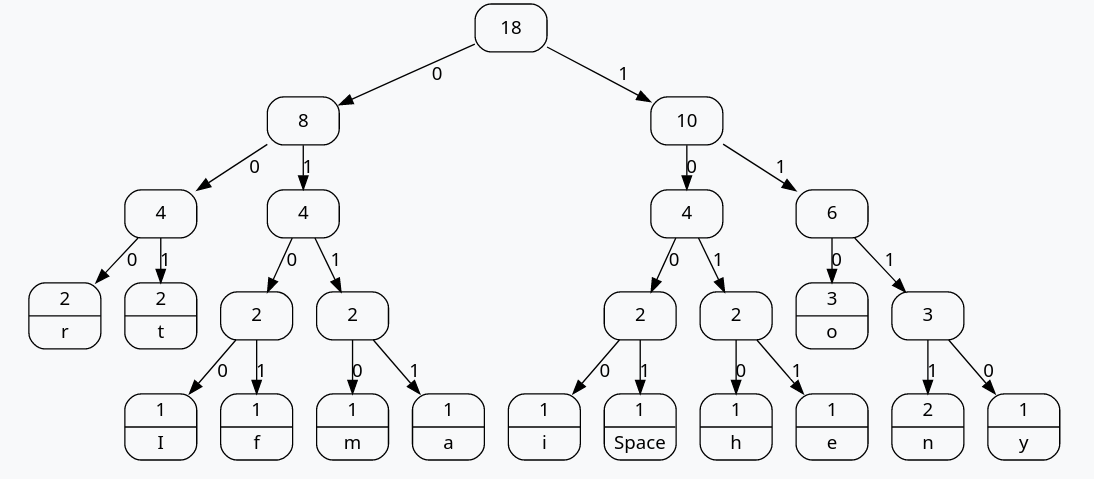
\includegraphics[width=0.5\linewidth]{images/HuffmanBT.png}
    \caption{Enter Caption}
    \label{fig:huffman-bt}
\end{figure}

By traversing this tree from node to node to reach the nodes corresponding to the letters we are looking for, we can find the compressed binary code assigned to them. The nodes on the left have a metric of 0 on their branch and a metric of 1 for the branches on the right (refer to the diagram of the previous tree). This gives the following binary code for the chosen source: \textbf{1101100100101110111101100100111011000011000000010111100} ... Much better, isn't it?

In order to decompress our compressed source and retrieve the exact starting data, we need to transmit the tree when communicating the source. (In Python we pass the object created for the tree).

As each node corresponds to a letter and has a weight on the branch linking it to other nodes, we can recover the exact source by simply traversing the tree and obtaining the \textbf{"Information theory"} string again.

\subsubsection{Limits and Performances}

For any source \textbf{X} with a Shannon entropy noted \textbf{H(X)} has an average length \textbf{L} of a codeword obtained by Huffman coding verified the following property: 

$H(X) <= L < H(X) + 1$.

The previous relationship shows that Huffman's algorithm approximates the entropy of our source and this may not be very interesting in the case of high entropy, where an overhead of 1 bit becomes significant. 

One solution to this problem is to work on blocks of \textbf{n} symbols. We then show that we can get closer to the entropy: 

$ H(X)\leq L<H(X)+{\frac {1}{n}} $

but the process of estimating probabilities becomes more complex and costly.
\subsection{Forward error correcting}

In telecommunications and computing, forward error correction (FEC) is a digital signal processing technique used to control errors in data transmission over unreliable or noisy communication channels, as well as to independently increase data reliability at the receiver to ensure high quality.

FEC improves bit error rate efficiency in communication systems, but involves additional digital processing, making it more expensive in terms of cost and spectral efficiency. The balance between these two elements needs to be taken into account in systems.

This is achieved by introducing redundant data using error-correcting codes (ECC) before the message is transmitted.  Without redundancy, every piece of data in the message is essential to its understanding. Any error in the message can therefore change its meaning.  The aim is to ensure that errors do not compromise the overall understanding of the message, and do not trigger a request for a re-transmission of the message by the receiver, thereby reducing channel traffic by more than a factor of two.

\subsubsection{Introduction to error correction code}

The problems encountered by modern industry are very diverse, all offering multiple techniques used for error-correcting codes. In some cases, such as data transmission over the Internet, the ECC's role is limited to error detection. In other cases, such as the TCP protocol on the transport layer of the OSI model, when an error is detected during message transmission, it is corrected by retransmitting the message. The techniques listed here are just a few of a sea of others, and today we're going to take a look at a very special technique known for its effectiveness : \textbf{Convolutional correctors}

The special feature of a convolutional ECC is that its output depends on the current symbol to be coded, as well as the previous symbol and the result of coding the previous symbol, unlike block codes, which process each block of information independently of the others.

For the purposes of this report, we will confine ourselves to the case of discrete communication channels, which are nothing other than binary channels transmitting only 0 or 1, i.e. bits of information.

\subsubsection{Convolutional encoding}

\begin{figure}[H]
    \centering
    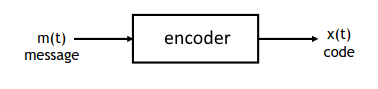
\includegraphics[width=0.5\linewidth]{images/encodeur_schem.png}
    \caption{Communication encoder diagram}
    \label{fig:encoder-diagram}
\end{figure}

A convolutional encoder is a finite state machine, and its state diagram can be represented as a lattice (the temporal equivalent of a state diagram). All states are arranged in columns to represent a state at time \textbf{t}, where \textbf{m(t)} and \textbf{x(t)} are discrete signals whose samples are binary. These states are linked to the same sets of states representing time t+1, in accordance with the transition table.

\begin{figure}[H]
    \centering
    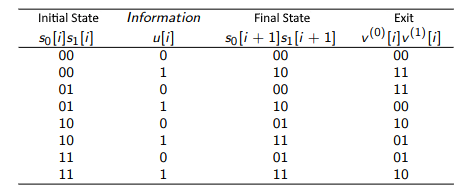
\includegraphics[width=0.5\linewidth]{images/transitionTable.png}
    \caption{Transition table with i for the clock time}
    \label{fig:transition-table}
\end{figure}

If the encoder is a linear system, \textbf{x(t)} can be generated by a convolution product:
\[ x_{j} = \sum_{i=0}^M g_{i}m_{j-i} \]

In order to carry out a binary convolution coding we will set some parameters:
\begin{itemize}
     \item $g_{i} = 0 \rightarrow$ connection absent
     \item $g_{i} = 1 \rightarrow$ connection present
     \item $K \rightarrow$ Constraint length (number of sampling instants during which a message bit participates in the elaboration of the output)
\end{itemize}

This is a so-called sliding window coding where there are two integers \textit{m} (for memory) and \textit{a} (for anticipation) such that the index symbol n of the coded sequence depends only on the finite source block between the indices $n - m$ and $n + a$.
\begin{figure}[H]
    \centering
    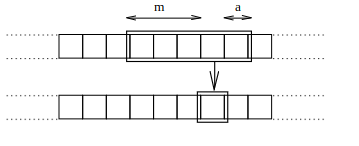
\includegraphics[width=0.5\linewidth]{images/register.png}
    \caption{Shift register}
    \label{fig:shift-register}
\end{figure}

For 1/2-rate 2-memory convolutional encoder we take M = 2, then we have K = M + 1 = 3 with an output interleaving n = 2, so using the above formula we obtain the following generator polynomials: $g_{1} = [1, 1, 1]$ and $g_{2} = [1, 0, 1]$.

All these parameters allow us to obtain the following logic diagram, enabling convolutional coding of our ECC: 
\begin{figure}[H]
     \centering
     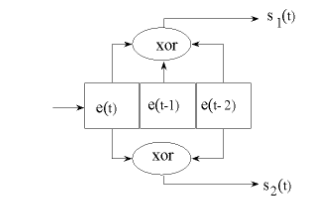
\includegraphics[width=0.5\linewidth]{images/logical_circuit.png}
     \caption{Data transmission in a convolutional encoder with a shift register and exclusive ORs}
     \label{fig:logical-circuit}
\end{figure}

Using this schema and XORing according to the connections said to be absent or present on the register undergoing a shift along the chain to be encoded we obtain:
\begin{itemize}
 \item Initial string : \textbf{1010}
 \item Encoded string: \textbf{11100010}
\end{itemize}

We therefore observe the presence of redundancy, as explained in the introduction, with a redundancy bit for each bit of the initial character string, which we'll use for decoding.

Before we start decoding, as we are working on noisy discrete channels, we will apply noise to the character string to check that our appended code is working correctly. Our message therefore becomes $\rightarrow$ \textbf{11100011}


\subsubsection{Decoding with Viterbi algorithm}

The Viterbi algorithm is based on the dynamic programming paradigm. We start from a starting state (default 00) and seek to find the path from the starting state whose output has the same length and is as close as possible to the message to be decoded. To apply this notion of proximity, we use the Hamming distance, which counts the number of different bits between two messages of the same finite or infinite length. 

This Hamming distance can be translated into the following pseudo-code:

\begin{algorithm}[H]
\begin{algorithmic}
\Function{Hamming distance}{$\text{s1}, \text{s2}$}
    \If{$\text{len}(\text{s1}) \neq \text{len}(\text{s2})$}
        \State \Return "Strings must be of equal length"
    \EndIf
    \State $\text{dist} \gets 0$
    \For{$i \gets 0$ \textbf{to} $\text{len}(\text{s1}) - 1$}
        \If{$\text{s1}[i] \neq \text{s2}[i]$}
            \State $\text{dist} \gets \text{dist} + 1$
        \EndIf
    \EndFor
    \State \Return $\text{dist}$
\EndFunction
\end{algorithmic}
\end{algorithm}

In response to the dynamic programming paradigm, the Viterbi algorithm can be represented in ways other than as a lattice. For the sake of simplicity, it will be presented in the form of a binary tree, so that we can create a history of all possible paths and perform a recursion to calculate the metric of each path from that of each branch, and reconstruct the message to be decoded.

\begin{figure}[H]
     \centering
     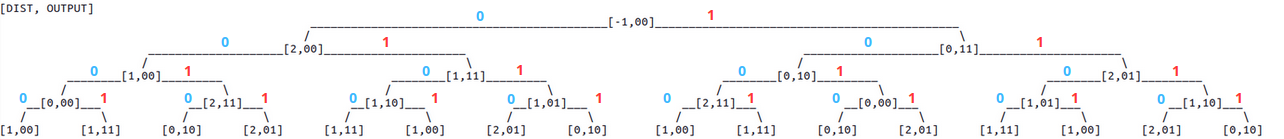
\includegraphics[width=1\linewidth]{images/BT_ECC_CV.png}
     \caption{Representation of the binary tree of the Viterbi lattice}
     \label{fig:bt-ecc-cv}
\end{figure}

Using the transition table in figure n°\ref{fig:transition-table}, we can move from one state to another and retrieve the new state, as well as the output bits, all thanks to the input bits which are 0 for the nodes on the left and 1 for the nodes on the right. A state is in fact a pair of bits resulting from the concatenation of the initial bit and the redundancy bit. If we go back up our tree, all we have to do is concatenate the input bits to reconstitute the message, even if it has been noisy. We know which is the safest path to take thanks to the distances noted above.

\begin{figure}[H]
     \centering
     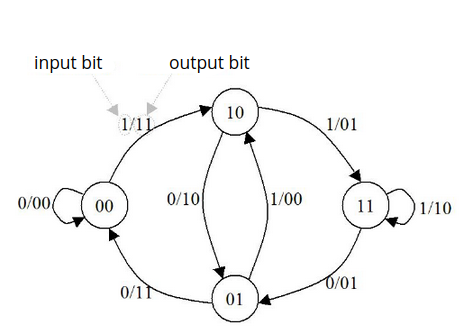
\includegraphics[width=0.5\linewidth]{images/logical_circuit_v2.png}
     \caption{State diagram of a convolutional encoder with 2 memories and 1/2 rate}
     \label{fig:logical_circuit_v2}
\end{figure}

Now, we can retrieve the correct message that is \textbf{1010}.

\newpage
\subsection{Cryptography}
\subsubsection{Introduction}
In a traditional definition of security of a cryptography scheme, one usually defines a game that characterizes the capabilities of a (hypothetical) adversary. A cryptography scheme is defined to be secure if no computationally feasible strategy allows the adversary to win the game with non-negligible probability (or advantage), for reasonable notions of feasible and negligible.
\cite{maurer2011constructive}

\paragraph{Important Elements of Cryptography}
\paragraph{Plain-text}
Original text that is immediately intelligible and can therefore be directly, without the need for deciphering.
\cite{ramet_r3.09}

\paragraph{Encrypting}
An operation that substitutes a plain text with an unintelligible text that cannot be understood by anyone who does not possess the key. Inoperable by anyone who doesn't have the key.

\paragraph{Ciphertext}
Message made unintelligible through encryption, which can only be and used only by those in possession of the encryption key.

\paragraph{Decryption}
Reverse operation of a reversible encryption, allowing an authorized in possession of the key, to restore a ciphertext in clear text.

\paragraph{Types of Cryptography}
There are two types of Cryptography: symmetric key Cryptography and asymmetric key Cryptography, both still in use today, but they have different applications due to their different qualities.

\paragraph{Symmetric Cryptography}
Symmetric Cryptography is the first one to appear, as it is a basic concept, it is as if we had a key to open a chest. In Cesar cipher is the number of shifts we will do on the alphabet to write and read the plain-text and the ciphertext respectively. The key being the most essential element in computational Cryptography, it can be almost anything that is information, a string of text, numbers, an image, etc… That information being processed by a Cryptography algorithm it can then encode or decode Cryptographic data. Today symmetric Cryptography is used in cases where we need fast service using not much resources and not needing to share the secret key often. Such qualities interest banks for example. There are multiple symmetric cryptography algorithms such as AES, DES, 3DES, and Blowfish. All of them are based on the Feistel Network except for AES which uses a Substitution and Permutation Network.

\paragraph{Asymmetric Cryptography}
ECC (Elliptic-curve-Cryptography) Elliptic Curve Cryptography Overview Elliptic Curve Diffie Hellman A 384 bits ECC key has the same level of security as a 7680 bit RSA key, it is considered to be a Top Secret level of security by many governments such as the USA Government Shannon Information Theory and Cryptography.

\subsubsection{Advanced Encryption Standard (AES)}
AES was invented by two Belgians, Joan Daemen and Vincent Rijmen in 1998 and submitted to the National Institute of Standards and Technology (NIST) in 2001 in order to replace the DES (Data Encryption Standard) which was starting to get outdated. It uses a key of 3 different lengths 128, 192, and 256 bits.
\cite{wiki_aes}


\paragraph{Variables}\cite{nist_aes}
\begin{itemize}
    \item [$-$] \textbf{state} Intermediate result of the AES block cipher that is represented as a two-dimensional array of bytes with four rows and Nb columns.
    \item [$-$] \textbf{keys} the key schedule generated by the key expansion algorithm
\end{itemize}
\paragraph{Constants}\cite{nist_aes}
\begin{itemize}
    \item [$-$] \textbf{s\_box} A non-linear substitution table used in SUBBYTES and KEYEXPANSION to perform a one-to-one substitution of a byte value.
    \item [$-$] \textbf{inv\_s\_box} A non-linear substitution table with the inverse values of the S-box used for the decryption.
    \item [$-$] \textbf{mix\_columns} A fixed matrix used on the MIXCOLUMNS
    \item [$-$] \textbf{inv\_mix\_columns} The matrix with the hexadecimal values of mix\_columns used in INVMIXCOLUMNS
    \item [$-$] \textbf{rcon} Is the key expansion round constants used on the KEYEXPANSION
\end{itemize}
\paragraph{Functions}\cite{nist_aes}
\begin{itemize}
    \item [$-$] \textbf{SUBBYTES} Takes the state as the parameter and applies the s\_box to each byte independently.
    \item [$-$] \textbf{SHIFTROWS} Takes the state as the parameter and transforms the state shifting the last three rows with different offsets (2nd row has 1 offset, 3rd row has 2 offsets, and 4th row has 3 offsets)
    \item [$-$] \textbf{MIXCOLUMNS} Takes the state as the parameter and each column is multiplied by the Mix Columns matrix. But the multiplication is done in the Galois Field. Which means that the sum is done with the XOR operation and the multiplication is done with the AND operation.
    \item [$-$] \textbf{KEYEXPANSION} Takes the key as the parameter, the routine that generates the round keys from the key.
    \item [$-$] \textbf{ADDROUNDKEY} Takes the state and round key as the parameters and transforms the state by performing an XOR operation on the state with the round key.
    \item [$-$] \textbf{CIPHER} Takes the plain text and the key as arguments and perform the AES algorithm using the functions SUBBYTES, SHIFTROWS, MIXCOLUMNS, KEYEXPANSION and ADDROUNDKEY.
    \item [$-$] \textbf{INVCIPHER} Takes the cipher text and makes the reverse operation as CIPHER.
\end{itemize}

\paragraph{AES Algorithm}\cite{nist_aes}
\begin{algorithm}[H]
\caption{CIPHER Algorithm}
\begin{algorithmic}[1]
\Procedure{CIPHER}{$plain\_text: list[int], key: list[int]$}
    \State $state \gets 4 \times 4$ matrix of zeros
    \For{$i \in [0, 4)$}
        \For{$j \in [0, 4)$}
            \If{$i*4+j < \text{len}(plain\_text)$}
                \State $state[j][i] \gets plain\_text[i*4+j]$
            \EndIf
        \EndFor
    \EndFor
    \State $keys \gets \text{KEYEXPANSION}(key)$
    \State $state \gets \text{ADDROUNDKEY}(state, keys[0])$
    \For{$i \in [1, 10)$}
        \State $state \gets \text{SUBBYTES}(state)$
        \State $state \gets \text{SHIFTROWS}(state)$
        \State $state \gets \text{MIXCOLUMNS}(state)$
        \State $state \gets \text{ADDROUNDKEY}(state, keys[i])$
    \EndFor
    \State $state \gets \text{SUBBYTES}(state)$
    \State $state \gets \text{SHIFTROWS}(state)$
    \State $state \gets \text{ADDROUNDKEY}(state, keys[10])$
    \State \Return $[state[i][j] \text{ for } i \in [0, 4) \text{ for } j \in [0, 4)]$
\EndProcedure
\end{algorithmic}
\end{algorithm}

\paragraph{Why is AES so hard to break}
For symmetric Cryptography we have three properties that measures if a cryptography system is secure or not.
\paragraph{Confusion and Diffusion}\cite{ramet_r3.09}
Confusion is when there is no statistical property that can be deduced from the ciphertext and Diffusion is when a change on the plain text changes the majority of the ciphertext.

\paragraph*{Example of Diffusion and Confusion in AES}

\textbf{Plain-text 1:} Hello World!

\textbf{Ciphertext 1:} \\
{\small\texttt{0101111111001111111111000010100001101100110001011011001010001000\\1110101000000011000011101000100010011000110110001100011001000010}}

\textbf{Plain-text 2:} Hallo World!

\textbf{Ciphertext 2:} \\
{\small\texttt{0100011001111001011111000100101000100100010011110101001100010100\\1011001010110010110110001010010101111111101101011110011110100111}}

\paragraph*{Analysis}

As observed, changing one letter in the plain-text resulted in a completely different ciphertext. This demonstrates the \textbf{Diffusion} property of AES. Moreover, due to the significant changes in the ciphertext, it becomes challenging to deduce statistical properties from these two messages, showcasing the \textbf{Confusion} property.

\paragraph{Key robustness} 
When is hard to find or enumerate all possibilities of key.

If the algorithm has the Diffusion and the Confusion properties, the only way to find the key would be by trying every combination of key. Which means that to find the key it would be needed to try 2 to the power 128 possibilities.

\paragraph{Why is AES better than DES}
\begin{itemize}
    \item AES provides stronger security compared to DES.
    \item AES is faster and more efficient in terms of computation compared to DES.
    \item AES has been subjected to more scrutiny and analysis than DES, making it more reliable.
\end{itemize}

\subsubsection{Elliptic-curve Cryptography (ECC)}
ECC (Elliptic-curve Cryptography) is a public-key cryptography algorithm based on the algebraic structure of elliptic curves over finite fields. It offers a high level of security with relatively short key sizes compared to other public-key cryptography algorithms like RSA. Elliptic Curve Diffie-Hellman (ECDH) is a key exchange protocol based on ECC, and it provides a secure way for two parties to establish a shared secret over an insecure channel. Although ECC is more secure than RSA, a 384 bit ECC key is equivalent to a 7680 RSA key for example.

\paragraph{How does Elliptic-curve Cryptography works}\cite{pierce_ecdh}
\paragraph{Curve}
An Elliptic-curve is defined by 
\begin{equation*}
y^2 = x^3 + ax + b
\end{equation*}
where $a$ and $b$ are constants. And the curve looks like this.

\begin{figure}[H]
\begin{minipage}{0.5\textwidth}
  \centering
  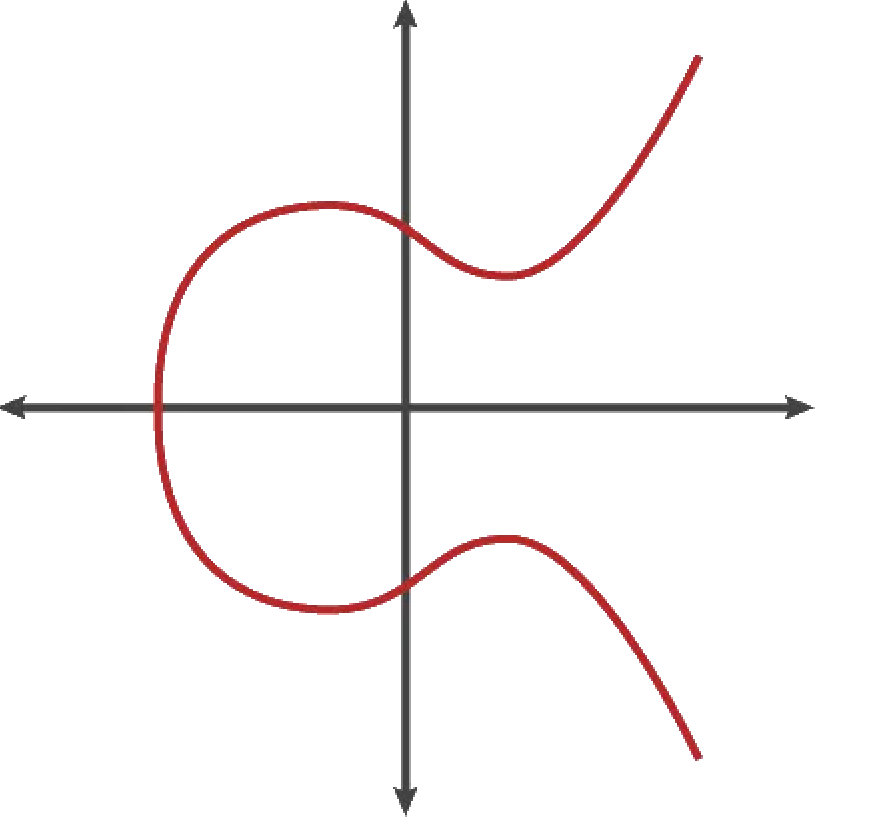
\includegraphics[width=\linewidth]{images/curve.png}
  \caption{Elliptic-curve.}
  \label{fig:Elliptic curve}
\end{minipage}%
\begin{minipage}{0.5\textwidth}
An Elliptic-curve is defined by $y^2 = x^3 + ax + b$ where $a$ and $b$ are constants. This figure illustrates the general shape of an elliptic curve.
\end{minipage}
\end{figure}

\paragraph{Addition}
The addition operation consists of finding a 3rd point on the curve. In the example we see the following operation:
\begin{equation}
P + Q = R
\end{equation}
When we draw a line that passes through $P$ and $Q$ we get $-R$ and through the property of symmetry of elliptic curves, we can find $R$.

\begin{figure}[H]
\begin{minipage}{0.5\textwidth}
  \centering
  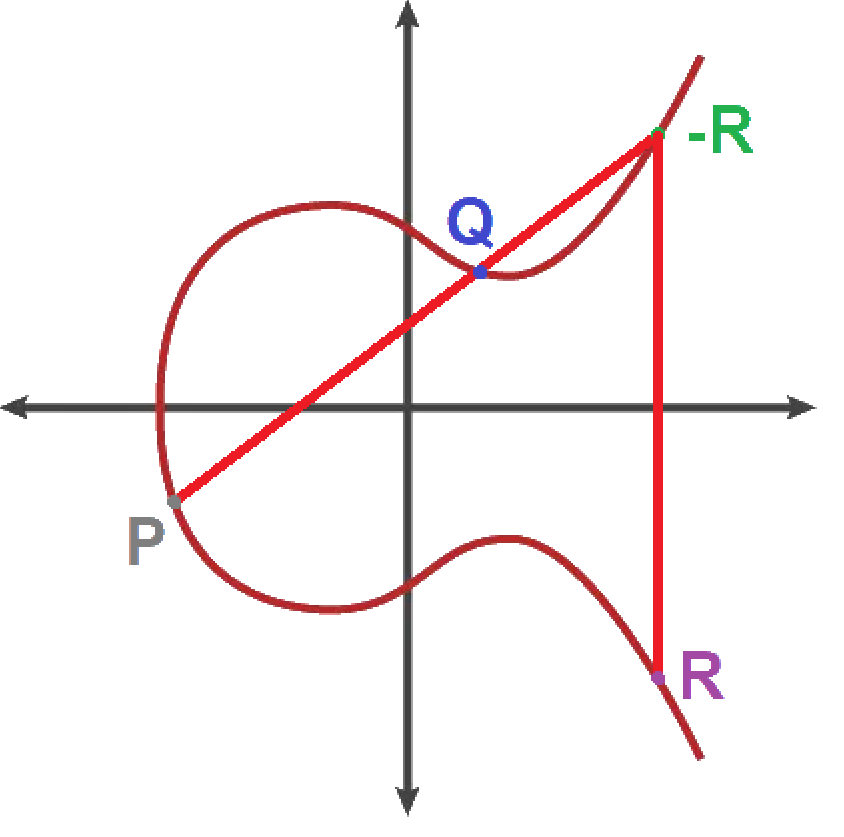
\includegraphics[width=\linewidth]{images/point_addition.png}
  \caption{Point addition in ECC.}
  \label{fig:point addition in ECC}
\end{minipage}%
\begin{minipage}{0.5\textwidth}
The addition operation consists of finding a third point on the curve. This figure illustrates the geometric interpretation of point addition in ECC.
\end{minipage}
\end{figure}

\paragraph{Multiplication}
The multiplication operation consists of adding a point $k$ times.
\begin{equation}
kP = P + P + \ldots + P 
\end{equation}
When adding a point to itself on a curve, the line drawn is the tangent to the curve at that point, $P$.

\begin{figure}[H]
\begin{minipage}{0.5\textwidth}
  \centering
  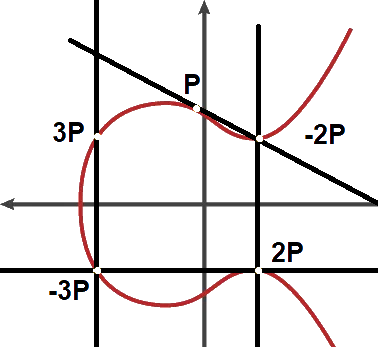
\includegraphics[width=\linewidth]{images/mult.png}
  \caption{Scalar Multiplication.}
  \label{fig:Scalar Multiplication}
\end{minipage}%
\begin{minipage}{0.5\textwidth}
The multiplication operation consists of adding a point $k$ times. This figure illustrates the concept of scalar multiplication in ECC.
\end{minipage}
\end{figure}

\paragraph{Implementation}
We will need to Implement two functions, add (make the addition of points), multiply(multiply a point).

The multiplication function will be a simple function of repeating an addition n times.
For the addition it wont be as simple.
So the algorithm will implement this logic.
\begin{enumerate}
    \item If one of the points is the point at infinity (represented as (0, 0)), then adding it to another point returns the other point.
    \item If the points are additive inverses (negatives) of each other, their sum is the point at infinity.
    \item If the points are distinct, calculate the slope of the line passing through them.
    \begin{equation}
    s = \frac{{Y_P - Y_Q}}{{X_P - X_Q}}
    \end{equation}
    \begin{equation}
    X_R = s^2 - (X_P - X_Q)
    \end{equation}
    \begin{equation}
    Y_R = s(X_P - X_R) - Y_P
    \end{equation}
    \item If the points are the same, calculate the slope of the tangent line to the curve at that point.
    \begin{equation}
    s = \frac{{3X_{P}^{2} + a}}{{2Y_{P}}}
    \end{equation}
    \begin{equation}
    X_R = s^2 - 2X_P
    \end{equation}
    \begin{equation}
    Y_R = s(X_P - X_R) - Y_P
    \end{equation}
\end{enumerate}

\begin{algorithm}[H]
\caption{Add two points on the curve}
\begin{algorithmic}[1]
\Procedure{Add}{$p, q$}
    \If{$p = (0, 0)$}
        \State \textbf{return} $q$
    \EndIf
    \If{$q = (0, 0)$}
        \State \textbf{return} $p$
    \EndIf
    \If{$p[0] = q[0]$ \textbf{and} $p[1] = -q[1]$}
        \State \textbf{return} $(0, 0)$
    \EndIf
    \If{$p \neq q$}
        \State $l \gets (q[1] - p[1]) \cdot (q[0] - p[0])^{-1} \mod p \, \% \, p$
    \Else
        \State $l \gets (3 \cdot p[0]^2 + a) \cdot (2 \cdot p[1])^{-1} \mod p \, \% \, p$
    \EndIf
    \State $x \gets (l^2 - p[0] - q[0]) \mod p \, \% \, p$
    \State $y \gets (l \cdot (p[0] - x) - p[1]) \mod p \, \% \, p$
    \State \textbf{return} $(x, y)$
\EndProcedure
\end{algorithmic}
\end{algorithm}

\paragraph{What makes ECC secure}

For a asymmetric Cryptography system the most important thing is to create a common key between two parts while not revealing their own private key, so it must be easy to calculate a public key from the private key but hard to make the reverse operation from the public key, that is called a trapdoor function.

To show how ECC works let's try a practical example:
\begin{figure}[H]
  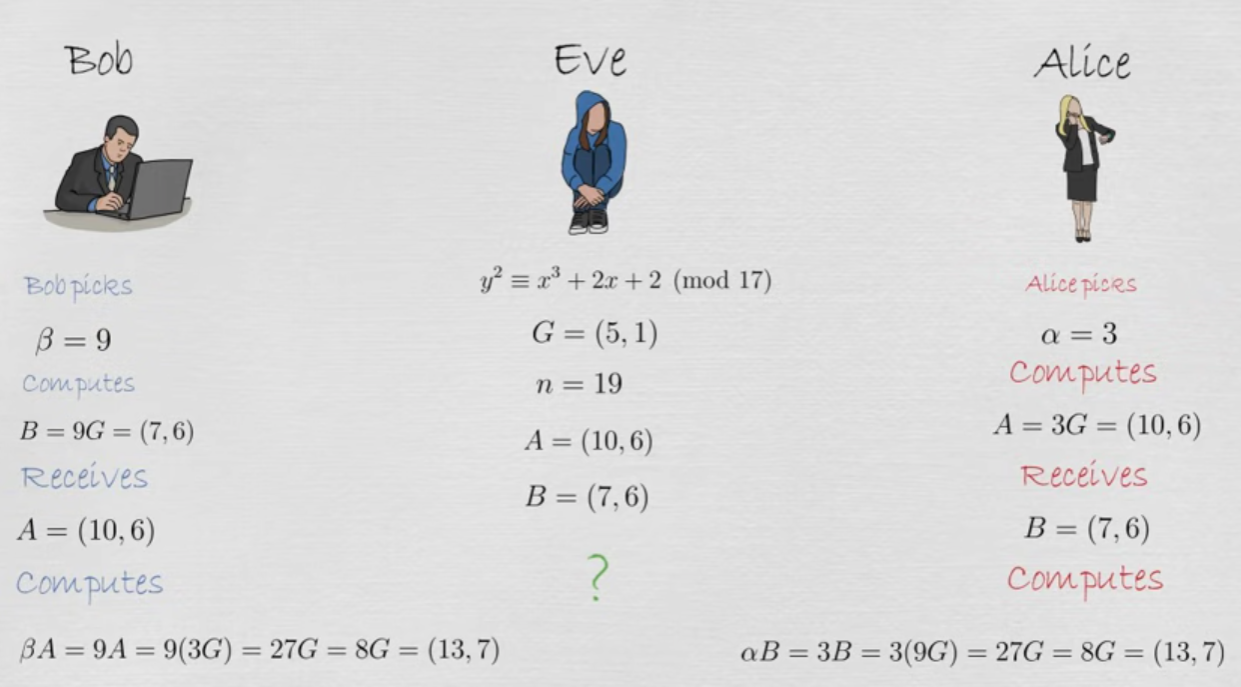
\includegraphics[width=\linewidth]{images/expl.png}
  \caption{Practical example of ECC.}\cite{pierce_ecdh}
  \label{fig:Practical example of ECC}
\end{figure}
In this scenario, Eve, acting as the intermediary, managed to obtain some information, albeit incomplete. However, she lacks the critical data necessary to compute the private keys. The inherent complexity of elliptic curves ensures that deriving either the private key $\beta$ (Bob's private key) or the private key $\alpha$ (Alice's private key) in ECC solely from a point on the curve is highly challenging.
This is a simple example, as there are standard parameters for the curb such as sect571k1. \cite{secg2010}


\subsubsection{Cryptography and Shannon Information Theory} \cite{shannon1948mathematical}

In The Theory of Communication the encoding and decoding are operations made by the transmitter and the receiver both will be called transducers.

And according to the Theorem 9 it is not possible for the channel to transmit at an average rate greater than: $\frac{C}{H}-\epsilon$

For the AES cryptography system the limit is calculated like this:

First let's calculate the capacity C of the system.
As in ASCII we have a set of characters of length 128, let's name it A* and every character (or symbol) is coded in 7 bits they have the same time of encoding or decoding.
Let's define \textbf{z} which is theoretical time that a transducer takes to encode or decode a character
\begin{enumerate}
    \item Build the system for the calculations
        \begin{figure}[H]
          \centering
          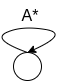
\includegraphics[width=0.15\linewidth]{images/system.png}
          \caption{cryptosystem schema.}
          \label{fig:cryptosystem}
        \end{figure}
        The matrix defining the system above will look like:
        $\left|({128*W^{z}})-1\right| = 0$
    \item Find the determinant of the equation, in this case as the matrix is a singleton matrix, the determinant of the matrix is itself.
    \item Solve ${128*W^{z}}-1 = 0$ to find $W$
    \item Calculate the capacity $C = logW$
\end{enumerate}

Secondly, H is defined as the bits per symbol as said before:
$H = 7$

Finally calculate the maximum average rate of the channel $\frac{C}{H}$
\begin{equation}
    \frac{logW}{7}
\end{equation}
\newpage

\section{Conclusion}

The Theory of Communication of Shannon showed to be a useful tool of prediction, on the WORD GAME where it is used to predict the path with the
most possibilities to find a specific word between a set of words or measuring
the maximum of information that can flow in a communication channel.

\newpage
\include{sections/annexes}

\end{document}